\section{Results}\label{sec:results}

\subsection{Estimating the scaling rate from sparse labels}\label{sec:estimation}

Table~\ref{tab:ablation} compares the hybrid sensor with its kinetic
core and with a purely data-driven model on the unseen test windows.
\begin{table}[t]\centering
\caption{Estimation on unseen test windows: RMSE in
$\log(1{+}\cdot)$ rate space (mean $\pm$ sd over \NUM{T1plants} plant
realizations) and the fraction of estimates within a factor of two of
the hidden truth. Generated from
\texttt{results/table1\_summary.csv}.}
\label{tab:ablation}
\begin{tabular}{lccc}
\toprule
Estimator & RMSE$_{\log 1p}$ & vs.\ physics & within $\times 2$ \\
\midrule
% GENERATED by manuscript/make_numbers.py — do not edit
Physics core & $0.346 \pm 0.181$ & --- & 41\% \\
Pure ML & $0.258 \pm 0.069$ & $-25\%$ & 64\% \\
Hybrid & $0.170 \pm 0.037$ & $-51\%$ & 84\% \\

\bottomrule
\end{tabular}
\end{table}
The hybrid reduces error by \NUM{T1redPh}\% against its physics prior
and by \NUM{T1redMl}\% against the data-driven model, and it places
\NUM{T1Hywf}\% of its estimates within a factor of two of the hidden
truth, against \NUM{T1Phwf}\% and \NUM{T1Mlwf}\%. Fig.~\ref{fig:scarcity}
shows how few labels this takes. With \NUM{ScDayMin} days of labels the
hybrid (\NUM{ScHyMin}) already outperforms the physics core given any
amount of data (at best \NUM{ScPhBest}) and the data-driven model given
all \NUM{ScDayMax} days (\NUM{ScMlMax}). A transfer test bounds the
claim: a residual carried to another plant together with its donor's
credibility does harm (\NUM{TrHy} against \NUM{TrPh} for the physics
prior, mean over \NUM{TrPlants} unseen plants), which is why $\lambda$
must be earned from the target plant's own labels. With no labels,
$\lambda = 0$ and the sensor is its prior.

\begin{figure}[t]\centering
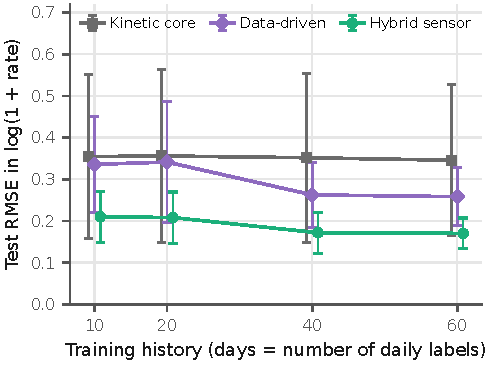
\includegraphics[width=.62\linewidth]{fig_paper_scarcity}
\caption{Estimation error versus the number of daily labels. Test RMSE
in $\log(1{+}\text{rate})$ of the kinetic core, the data-driven model and
the hybrid sensor; mean $\pm$ sd over \NUM{T1plants} plant realizations,
with points offset horizontally for legibility. Generated from
\texttt{results/scarcity\_sweep.csv}.}\label{fig:scarcity}
\end{figure}

The same correction pattern was replayed on laboratory truth
(Fig.~\ref{fig:sensorval}). Each of the \NUM{SvN} decay experiments of
\citet{scott2024silica} at pH 5--8 that consumed at least half of its
supersaturation and yields at least six usable rate intervals is treated
as a plant, with interval-average observed rates as the hidden truth,
the fitted core as the prior and only the first $K$ intervals as labels.
Three corrections with honestly counted parameters are compared: none,
that is the core alone; a one-parameter offset in log space, which can
be fitted from a single label where a data-only model cannot operate at
all; and a two-parameter affine correction whose slope in $\ln s$ is, by
construction, a correction of the reaction order. Second-order truth
against a fourth-order core predicts a slope $b \approx -2$. Fitted
without restraint, the affine correction fails: early labels span almost
no supersaturation (a spread in $\ln s$ of 0.047 against 2.61 over the
test window), the fitted slopes range from \NUM{SvAffMin} to
\NUM{SvAffMax}, and the correction does far worse than none. Under the
same credibility rule as the field sensor, a leave-one-out choice
between the offset and a clipped affine correction, the method keeps
the offset until the labels support a slope ($K \le 3$), and with one
to three labels the offset is level with the core (median RMSE
\NUM{SvOffLo}--\NUM{SvOffHi} against \NUM{SvPhysLo}--\NUM{SvPhysHi}). At
$K = 5$ the slope is adopted in \NUM{SvSelfive} of the \NUM{SvNfive}
experiments long enough to be scored, with a median $b =$~\NUM{SvBfive}
that independently recovers the second-order finding, and the
correction wins with a median RMSE of \NUM{SvCredfive} against
\NUM{SvPhysfive} for the core. The lesson carries over to the plant: a
correction should have no more freedom than the labels can identify,
and a line held near one operating point presents a level-dominated
problem in which a scalar correction is well identified.

\begin{figure}[t]\centering
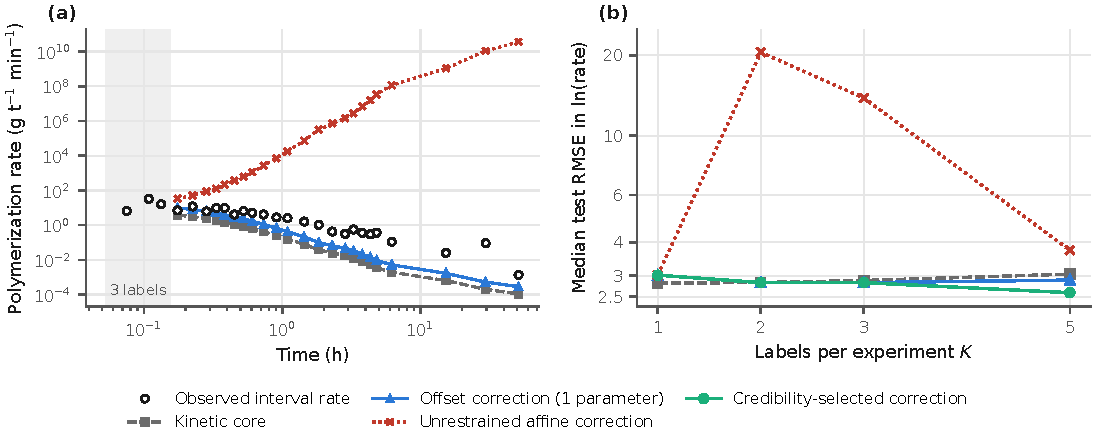
\includegraphics[width=\linewidth]{fig_paper_sensor}
\caption{The correction pattern on laboratory decay curves.
(a) Experiment \NUM{SvExp} of \citet{scott2024silica}
(\NUM{SvExpT}~$^{\circ}$C, pH \NUM{SvExpPH}) with three labels (shaded):
observed interval rates, the kinetic core, the one-parameter offset
correction, which with three labels is also the credibility-selected
correction, and the unrestrained affine correction, which diverges.
(b) Median test RMSE over the \NUM{SvN} experiments (\NUM{SvNfive} at
$K = 5$) versus the number of labels $K$. Source:
\texttt{results/sensor\_validation\_scott.csv}.}
\label{fig:sensorval}
\end{figure}

\subsection{The anchor of the correction decides safety}\label{sec:anchoring}

Table~\ref{tab:closedloop} gives the closed-loop results for fixed
practice, the open-loop robust policy and the scalar corrections, and
Fig.~\ref{fig:frontier} shows every policy as a trade-off between power
gain and violations; Table~S1 of the Supplementary material lists the
Gaussian-process and hybrid corrections in the same format.

\begin{table}[!tbp]\centering\footnotesize
\setlength{\tabcolsep}{3.2pt}\renewcommand{\arraystretch}{0.78}
\caption{Closed-loop results, mean over \NUM{CLplantsB} plant
realizations $\times$ \NUM{CLdays} days per regime. Gain is gross power
over fixed practice (mean $\pm$ sd over plants, \%). Violation days are
means per run with the worst plant in parentheses; ``post-w.'' counts
days after the 8-day warm-up. The scalar correction computed at the
measured silica without back-off is the $\kappa = 0$ row of the last
block. Generated from \texttt{results/table2\_summary.csv} and
\texttt{results/table2b\_summary.csv}.}
\label{tab:closedloop}
\begin{tabular}{lccccc}
\toprule
 & \multicolumn{2}{c}{Benign regime} & \multicolumn{3}{c}{Stress regime
 ($\times 6$)} \\
\cmidrule(lr){2-3}\cmidrule(lr){4-6}
Policy & Gain & Viol.\ days & Gain & Viol.\ days & Post-w. \\
\midrule
% GENERATED by manuscript/make_numbers.py — do not edit
Fixed practice & --- & 0.00 (0) & --- & 0.00 (0) & 0.00 \\
Robust optimum, no feedback & $+41.7 \pm 0.0$ & 0.45 (7) & $+41.7 \pm 0.0$ & 20.65 (28) & 17.50 \\
\addlinespace
\multicolumn{6}{l}{\emph{Anchoring ablation: scalar correction computed at}} \\
\quad design case, additive & $+81.5 \pm 20.7$ & 5.60 (17) & $+37.3 \pm 2.5$ & 15.80 (18) & 13.25 \\
\quad design case, log-space & $+100.3 \pm 33.5$ & 17.80 (21) & $+41.3 \pm 3.2$ & 19.20 (26) & 16.35 \\
\quad measured silica, log-space & $+3.4 \pm 52.2$ & 0.35 (2) & $-46.7 \pm 15.7$ & 0.25 (1) & 0.15 \\
\addlinespace
\multicolumn{6}{l}{\emph{Scalar correction at measured silica, back-off gain $\kappa$}} \\
\quad $\kappa = 0$ & $+40.6 \pm 7.1$ & 0.00 (0) & $+21.1 \pm 1.5$ & 1.60 (6) & 1.25 \\
\quad $\kappa = 0.5$ & $+34.8 \pm 6.1$ & 0.00 (0) & $+15.9 \pm 2.0$ & 0.65 (2) & 0.45 \\
\quad $\kappa = 1$ & $+29.3 \pm 5.6$ & 0.00 (0) & $+10.6 \pm 2.6$ & 0.40 (1) & 0.20 \\
\quad $\kappa = 2$ & $+18.6 \pm 6.6$ & 0.00 (0) & $-1.1 \pm 4.5$ & 0.25 (1) & 0.05 \\

\bottomrule
\end{tabular}
\end{table}

\begin{figure}[!tbp]\centering
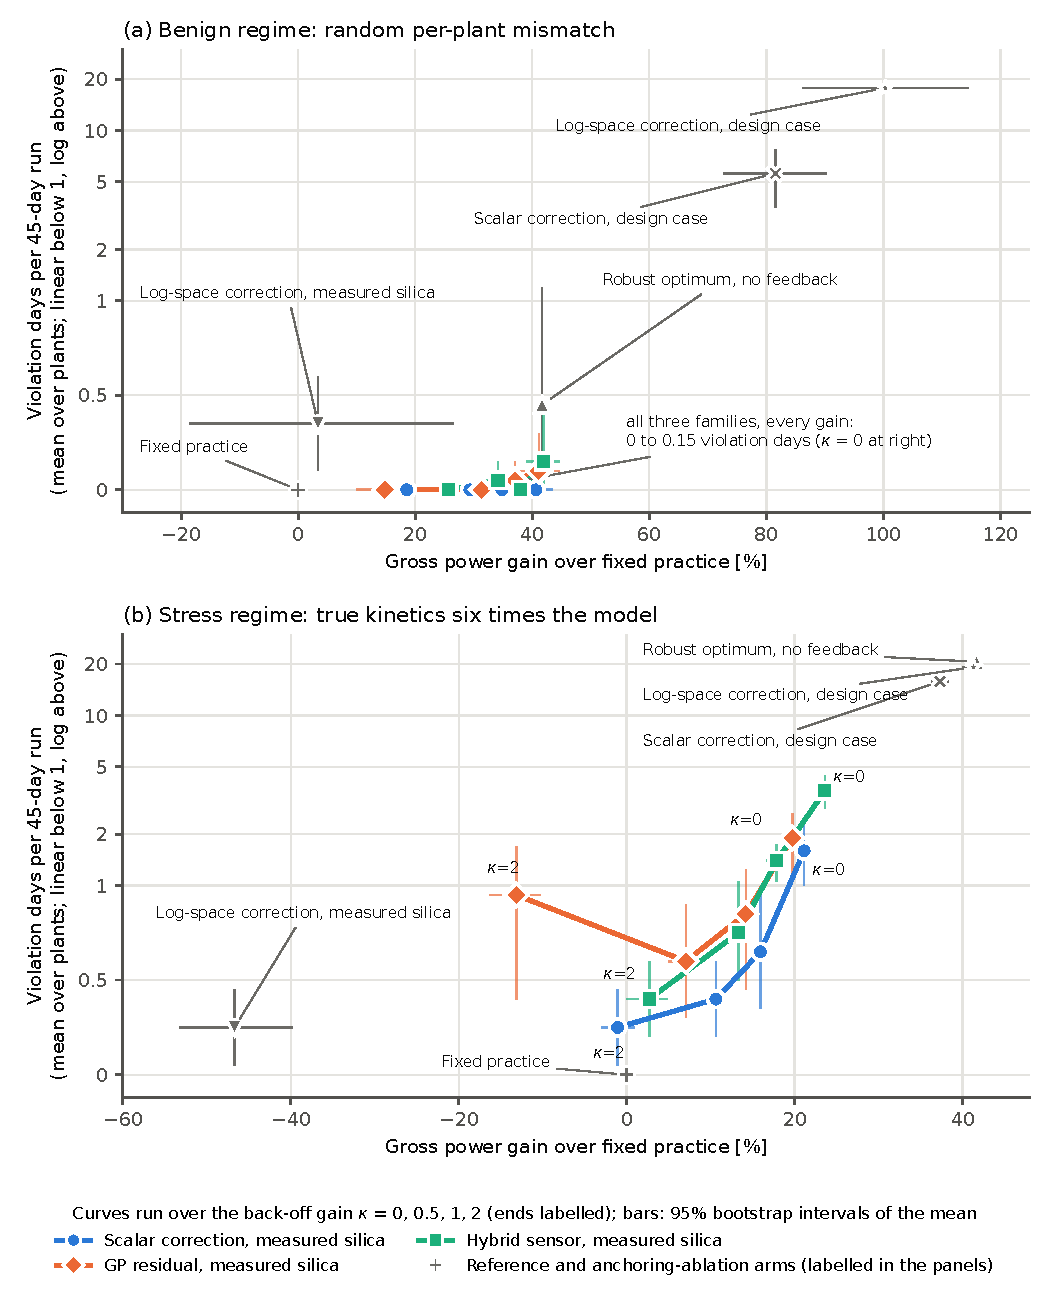
\includegraphics[width=\linewidth]{fig_closed_loop_frontier}
\caption{Trade-off between power gain and safety for every policy. Each
correction computed at the measured silica is a curve over the back-off
gain $\kappa = 0, 0.5, 1, 2$, with $\kappa = 0$ at the high-gain end;
fixed practice, the open-loop policy and the anchoring-ablation arms are
single labelled markers. Bars are 95\% bootstrap intervals of the mean
over plants. The vertical axis is linear below one violation day and
logarithmic above. Generated from
\texttt{results/closed\_loop\_frontier.csv}.}\label{fig:frontier}
\end{figure}

Consider the anchoring block of Table~\ref{tab:closedloop}. Computed at
the design case, the additive correction averages \CL{B}{CAnom}{v}
violation days per run in the benign regime (\CL{B}{CAnom}{m} on the
worst plant) and \CL{S}{CAnom}{v} in the stress regime, against
\CL{S}{Open}{v} with no feedback at all. Computed at the measured silica
concentration, the same correction at the same gain averages
\CL{B}{CAk0}{v} and \CL{S}{CAk0}{v}. The paired reductions are
\CT{anchorB}{v}{abs} days (95\% interval
\CT{anchorB}{v}{lop}--\CT{anchorB}{v}{hip}) and \CT{anchorS}{v}{abs}
days (\CT{anchorS}{v}{lop}--\CT{anchorS}{v}{hip}). The log-space
correction behaves the same way under stress, with \CL{S}{LGnom}{v}
against \CL{S}{LGmeas}{v} violation days.

A diagnostic isolates the mechanism. With the operating point held at
the open-loop optimum on the \NUM{AnPlants} stress plants, the model
error that a correction ought to see is a constant factor of six, and
the ratio of each day's label to the anchor model can be formed
directly. The design-case brine is more concentrated than the brine the
plant actually carries, so through the fourth-power rate law the
design-case model over-predicts the realized-brine model by a median
factor of \NUM{AnMarginmed}. That factor is the safety margin of the
robust optimizer. A correction computed at the design case sees the
product of this margin and the model error and cannot separate them.
Under the sixfold stress the two nearly cancel: the ratio of label to
design-case model has a median of \NUM{AnDesmed} (5th to 95th
percentile \NUM{AnDeslo}--\NUM{AnDeshi}), the correction finds almost
nothing to correct, and the line is left where the realized rate
exceeds the limit on \NUM{AnShare}\% of days. In the benign regime,
with no systematic kinetic error, the same correction reads the margin
as excess caution, relaxes the constraint, cools the line and violates.
Computed at the measured silica, the ratio has a median of
\NUM{AnMeasmed}, close to the kinetic error it should see.

That margin and stress are of nearly equal size here is a coincidence;
the confounding is not. Any scheme that is solved against a worst-case
envelope and corrected from plant feedback must compare the feedback
with the model at the realized conditions, or it will mistake its own
safety margin for model error, in whichever direction the two happen to
combine.

The diagnostic also explains why the log-space correction is so
cautious at the measured anchor. The measured-anchor ratio is
heavy-tailed (95th percentile \NUM{AnMeashi}) because on some days the
measured supersaturation is small and the model rate nearly vanishes.
An additive correction is insensitive to that tail, since a small model
rate yields a small absolute innovation; a multiplicative correction is
not, and under stress it ran the line hotter than fixed practice
(\CL{S}{LGmeas}{u}\% power).

\subsection{Correction model and back-off}\label{sec:models}

In the benign regime, once computed at the measured silica, all three
corrections are essentially free of violations. Without back-off the
scalar correction has no violation day on any of the \NUM{CLplantsB}
plants, the Gaussian-process residual averages \CL{B}{GPk0}{v} and the
hybrid \CL{B}{HYk0}{v}, at power gains of \CL{B}{CAk0}{u}\%,
\CL{B}{GPk0}{u}\% and \CL{B}{HYk0}{u}\%. These gains are those of the
open-loop robust policy (\CL{B}{Open}{u}\%), which nevertheless violates
on \CL{B}{Open}{v} days on average and \CL{B}{Open}{m} on its worst
plant, because an envelope over brine chemistry does not protect
against kinetic deviations. Here feedback buys safety rather than
power, and back-off costs power while buying nothing: $\kappa = 1$
takes \NUM{boCAB} points off the scalar correction's gain with no change
in violations.

In the stress regime the open-loop policy violates on \CL{S}{Open}{v}
days per run, and the three corrections separate into the curves of
Fig.~\ref{fig:frontier}(b). Without back-off the scalar correction keeps
a gain of \CL{S}{CAk0}{u}\% at \CL{S}{CAk0}{v} violation days. The
hybrid gains slightly more (\CL{S}{HYk0}{u}\%) and violates more
(\CL{S}{HYk0}{v} days; paired difference \CT{HYk0S}{v}{d}, interval
\CT{HYk0S}{v}{lop} to \CT{HYk0S}{v}{hip}). The Gaussian process gains
slightly less (\CL{S}{GPk0}{u}\%) at a violation count
indistinguishable from the scalar's (difference \CT{GPk0S}{v}{d},
interval \CT{GPk0S}{v}{lop} to \CT{GPk0S}{v}{hip}). Back-off moves each
family along its curve at a similar price. From $\kappa = 0$ to
$\kappa = 1$ the scalar correction gives up \CT{boCA}{u}{abs} points of
gain and \CT{boCA}{v}{abs} violation days, the hybrid
\CT{boHY}{u}{abs} points and \CT{boHY}{v}{abs} days, and the Gaussian
process \CT{boGP}{u}{abs} points and \CT{boGP}{v}{abs} days. At
$\kappa = 2$ the scalar and hybrid corrections are down to
\CL{S}{CAk2}{w} and \CL{S}{HYk2}{w} post-warm-up violation days, with
almost no gain left (\CL{S}{CAk2}{u}\% and \CL{S}{HYk2}{u}\%). Under a
sixfold kinetic error there is little extra power that is safe to take.

Read as curves, the families overlap, and no learned model dominates
the scalar correction. At equal gain the hybrid sits a few points of
power to the right of the scalar curve and somewhat above it (at
$\kappa = 1$: \CT{HYk1S}{u}{d} points, \CT{HYk1S}{v}{d} violation days),
which is a different point on a similar curve rather than a better
curve. The Gaussian-process family lies slightly inside the scalar one,
with less gain at every $\kappa$ and, at $\kappa = 2$, more violations
as well (\CT{GPk2S}{u}{d} points, \CT{GPk2S}{v}{d} days). A plausible
reason is that a wide posterior away from the visited operating points
pushes the optimizer into regions the model has not seen, the failure
that trust regions address in the Gaussian-process
literature~\citep{delriochanona2021tale}. Two further explanations are
offered, neither of which the experiments isolate. A line held near one
operating point needs a correction that is local and current, which a
scalar updated daily supplies and models refitted weekly do not. And
the hybrid's credibility shrinkage pulls its correction toward a
kinetic prior that, under stress, under-predicts sixfold; that protects
estimation accuracy but is the unsafe direction for control, and
without back-off the hybrid has the most violations of the three.

On the six plants of the registered protocol, the open-loop policy
violates chronically (\NUM{PreOpenv} days), as expected. The hybrid
without back-off averages \NUM{PreHYk0w} post-warm-up violation days,
missing its registered target of zero. The hybrid with $\kappa = 1$
averages \NUM{PreHYk1w} days against a registered criterion of at most
0.5, and it is safer than the arm without back-off, as registered. These
figures use the measured-anchored warm-up; with the original
design-case warm-up the two arms gave 2.17 and 0.50 days, and the
verdicts were the same.

\subsection{Operating points at the reinjection line}\label{sec:operating}

In plant terms the policies differ mainly in the reinjection
temperature they hold. Because gross power is linear in the temperature
drop (Eq.~\eqref{eq:power}), each plant's mean power gives its mean
reinjection temperature exactly, and its inhibitor cost gives its mean
dose. Fixed practice holds 150~$^{\circ}$C and 1~ppm. The open-loop
robust policy settles at \CL{B}{Open}{T}~$^{\circ}$C and
\CL{B}{Open}{dose}~ppm: lowering the line by \NUM{dTOpen}~K releases
\NUM{QthOpen}~MW of heat from the \NUM{Mflow}~kg/s stream, which the
assumed conversion effectiveness of \NUM{EtaB} turns into
\NUM{dMWOpen}~MW of additional gross power (\CL{B}{Open}{mw} against
\CL{B}{Fixed}{mw}~MW). In the benign regime the measured-silica
correction holds nearly the same point (\CL{B}{CAk0}{T}~$^{\circ}$C)
while removing the open-loop policy's violations, whereas the
design-case corrections cool the line to \CL{B}{CAnom}{T}~$^{\circ}$C
(additive) and \CL{B}{LGnom}{T}~$^{\circ}$C (log-space), which is where
their violations come from. In the stress regime the measured-silica
correction warms the line to \CL{S}{CAk0}{T}~$^{\circ}$C without
back-off and to \CL{S}{CAk1}{T}~$^{\circ}$C with $\kappa = 1$, while the
design-case correction stays at \CL{S}{CAnom}{T}~$^{\circ}$C, close to
the open-loop set-point. The safe response to sixfold faster kinetics
is a rise of \NUM{dTsafeA} to \NUM{dTsafeB}~K in reinjection
temperature, and the design-case correction does not find it.

The dose moves much less than the temperature. Across all optimized
policies and both regimes the mean dose lies between \NUM{DoseMin} and
\NUM{DoseMax}~ppm, below the 1~ppm of fixed practice, because the
inhibitor's suppression is flat near its optimum while its cost rises
linearly with dose. Inhibitor intensity falls from
\CL{B}{Fixed}{i}~PHP/MWh under fixed practice to \CL{B}{CAk0}{i}~PHP/MWh
under the measured-silica correction, partly through the lower dose and
mostly through the larger output over which the dose is spread.

\subsection{Sensitivity to kinetics, solubility, inhibitor response and
economics}\label{sec:sobol}

A Sobol study ($N = \NUM{SobN}$, seeded, \NUM{SobEvals} evaluations)
spans the declared uncertainty set of the open-loop optimum: a kinetic
band equal to the measured sixfold gap, the measured solubility band
$[0.90, 1.37]$, and scenario bands for the flash fraction (0.20--0.30),
the inhibitor response (maximum suppression 0.30--0.70, dose of maximum
effect 0.5--2.0~ppm), the scaling limit $r_{\max}$
(0.25--1.0~g\,t$^{-1}$\,min$^{-1}$), the conversion effectiveness
(0.08--0.14) and the electricity price (PHP~4--7/kWh)
(Fig.~\ref{fig:sobol}). Kinetic uncertainty dominates the open-loop
optimum, with total-order indices of \NUM{SobSTMw}, \NUM{SobSTT} and
\NUM{SobSTNet} on gross power, optimal temperature and net objective,
followed by solubility (\NUM{SobSTTce} on the optimal temperature). The
inhibitor response decides the dose and barely touches the temperature:
the dose of maximum effect has a total-order index of \NUM{SobSTDose}
on the optimal dose and \NUM{SobSTTdopt} on the optimal temperature,
and the maximum suppression has \NUM{SobSTTeta} on the optimal
temperature. Within the declared band, then, the assumed dose--response
family moves the dose that is chosen, not the reinjection temperature
or the power, and the benign regime already perturbs that response on
every plant (Section~\ref{sec:plant}). Feasibility holds at
\NUM{SobFeas}\% across the set. The gross-power optimum spans
\NUM{Sobmwq05}/\NUM{Sobmwq50}/\NUM{Sobmwq95}~MW
($q_{05}/q_{50}/q_{95}$); its median exceeds the nominal
\CL{B}{Open}{mw}~MW because several bands are not centred on the
nominal values and the study samples the flash fraction instead of
holding its adverse bound.

Re-valuing the closed-loop trajectories over the economic envelope
attaches ranges to every peso figure. The assumption that makes this
valid was checked rather than assumed: the optimum moves zero grid
steps across the eight corners of the envelope, with inhibitor cost
below 15\% of revenue everywhere, so power gains and violation counts
do not depend on the economic assumptions.

\begin{figure}[t]\centering
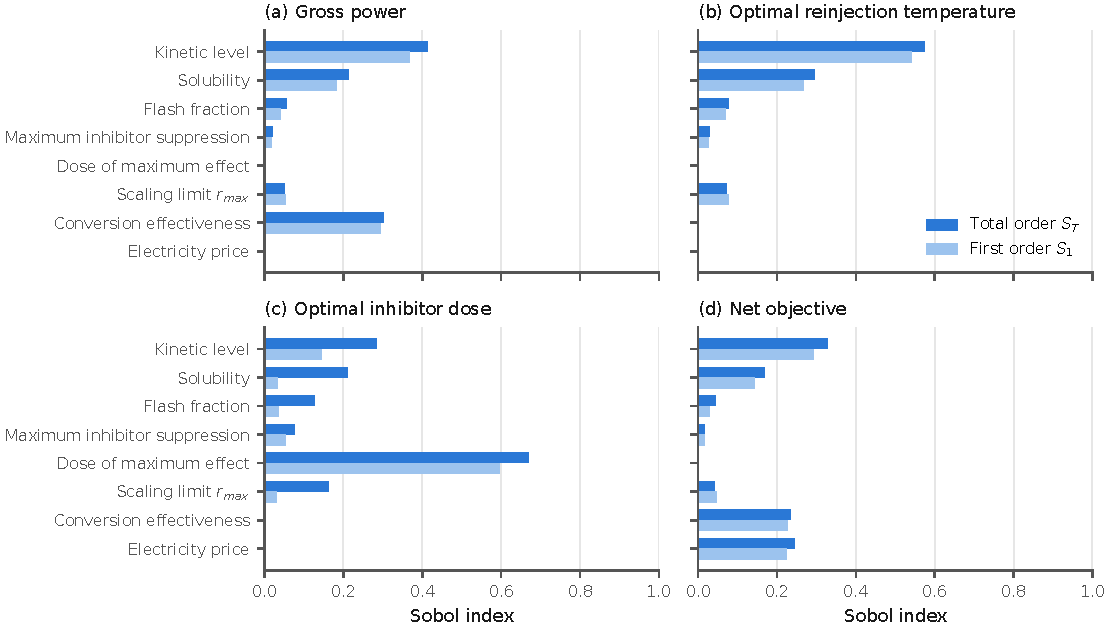
\includegraphics[width=\linewidth]{fig_paper_sobol}
\caption{Sobol sensitivity of the open-loop optimum. First-order
($S_1$) and total-order ($S_T$) indices of (a) gross power, (b) optimal
reinjection temperature, (c) optimal inhibitor dose and (d) net
objective over the declared uncertainty set. Generated from
\texttt{results/sensitivity\_sobol.csv}.}
\label{fig:sobol}
\end{figure}
